\documentclass[11pt,a4paper]{article}

\usepackage[margin=2.3cm]{geometry}
\usepackage{amsmath,amssymb}
\usepackage{graphicx}
\usepackage{booktabs}
\usepackage{array}
\usepackage{xcolor}
\usepackage{enumitem}
\usepackage[hidelinks]{hyperref}
\usepackage{caption}

\emergencystretch=1.5em
\captionsetup{font=small,labelfont=bf,width=.92\textwidth}
\setlength{\parskip}{4pt plus 1pt}
\setlength{\parindent}{0pt}

\newcommand{\code}[1]{\texttt{#1}}
\newcommand{\dv}[1]{diverged (#1)}

\title{Magnitude--direction decoupling versus its initialization\\[2pt]
\large Research note: attributing the advantage of MD training}
\author{}
\date{2026-09-21. Interim: 38 of 42 runs finished; in-progress cells are
marked and will be updated when the remaining runs complete.}

\begin{document}
\maketitle
\vspace{-2em}

% ============================================================
\section{Purpose and summary of conclusions}
% ============================================================

Magnitude--direction (MD) decoupled training changes two things at once: it
imposes a specific initialization, and it replaces the optimizer step with a
norm-constrained one. This note separates the two, to determine whether the
advantage of MD training over ordinary AdamW comes from the decoupled
optimizer itself or from the initialization it happens to impose.

The comparison is between full MD training and a new regime, \code{md\_init},
which starts from exactly the same initialization but then trains with the
ordinary AdamW. Each bottleneck family is run under full MD and under
\code{md\_init} with weight decay $0.1$ and $0.01$, over a grid of $(K,J)$
configurations at fixed temperature.

The main conclusions from the completed runs are:

\begin{itemize}[leftmargin=1.4em]
\item \textbf{Where training converges, the initialization accounts for most
of the final quality.} In every pair in which both regimes reached 20k steps,
\code{md\_init} lands within $0.001$--$0.041$ nats of full MD. Against the
better weight decay ($0.1$) the gap is $0.001$--$0.025$ nats. The gap favors
full MD in every comparable pair, in all three families.

\item \textbf{The decoupled optimizer itself contributes a stability margin.}
Full MD diverged only in rows in which every regime diverged ($K=128$ at
$T=1$, both surrogate families). \code{md\_init} additionally diverged in six
cells in which full MD converged. Where an entire row diverges, the order is
systematic: the $wd=0.01$ run dies first, $wd=0.1$ second, and full MD last.

\item \textbf{Within \code{md\_init}, weight decay $0.1$ dominates $0.01$.}
It reaches a lower final validation CE in every comparable pair and diverges
less often (two extra divergences versus four).

\item \textbf{Attribution.} The advantage of MD training decomposes into a
large initialization component, which ordinary AdamW inherits by starting
from the same weights, and a genuine optimizer component, which appears as a
small but consistent residual quality gap ($\lesssim 0.03$ nats at the
better weight decay) and, more prominently, as protection against divergence
at aggressive $(K,J,T)$ configurations.
\end{itemize}

% ============================================================
\section{The two regimes}
% ============================================================

\textbf{Full MD} (\code{model.decouple=true}). Every matrix weight is
optimized as a fixed-Frobenius-norm direction with learnable per-row and
per-column softplus gains; embedding rows are re-projected to unit L2 norm
after every step; no parameter receives weight decay. The initialization
draws every matrix entrywise $\mathcal N(0,1/d_{\mathrm{model}})$ and
projects it to Frobenius norm
$c_F=\sqrt{d_{\mathrm{out}}d_{\mathrm{in}}/d_{\mathrm{model}}}$; embedding
rows are drawn Gaussian and projected to unit L2 norm, with a fixed
$\sqrt{d_{\mathrm{model}}}$ upscale of the embedding output in the forward
pass.

\textbf{MD init} (\code{model.md\_init=true}, added for this comparison).
The identical initialization and the identical $\sqrt{d}$ forward upscale,
followed by ordinary AdamW: no gains, no re-projection after the step, and
the configured weight decay applies to every $\geq$2-D weight, embeddings
included. Weight decay $0.1$ matches this project's non-MD baseline runs;
$0.01$ probes the sensitivity to that choice.

\textbf{Initialization identity.} At equal seed the two regimes were
verified to start from bitwise-identical parameters at full size (all 66
parameter tensors of the 8$\times$768 model with the bottleneck spliced in,
checked in all three families) and to compute exactly equal forward logits
at initialization. Unit tests additionally verify that one optimizer step
leaves the norm constraints under \code{md\_init} and preserves them under
full MD. The comparison therefore isolates the optimizer step; nothing else
differs.

% ============================================================
\section{Setup}
% ============================================================

All runs use the 8$\times$768 architecture with tied embeddings, RoPE,
\code{abs\_topk} selection over $N=1536$ bottleneck features,
\code{residual\_out} placement, batch $96\times512$ tokens, lr $6\times
10^{-4}$ cosine with 500-step warmup, bf16, 20k steps, and one shared seed,
mirroring the earlier \code{uk} campaign configurations. Three bottleneck
families are compared:

\begin{itemize}[leftmargin=1.4em]
\item \textbf{Basic LapSum} (\code{rout\_soft}): hard Top-$K$ forward with
the mass-constrained LapSum surrogate at constant absolute $T$;
\item \textbf{RBLapSum} \code{through\_rank\_kappa} ($T$ fixed, boundary
floor $b_0=0.1$): the fully modified surrogate;
\item \textbf{Hard AbsTopK}: no surrogate gradient (active features only).
\end{itemize}

The grid is $(K,J)\in\{(32,32),(32,480),(128,128),(128,384)\}$ at $T=1$ for
the two surrogate families and $K\in\{32,512\}$ for the hard family. Because
every $K=128$, $T=1$ configuration diverged in both surrogate families under
every regime, the two $K=128$ pairs were rerun at $T=2$, where all regimes
can converge; these rows carry an explicit $T=2$ label. In total 42 runs.

A run is stopped and recorded as diverged when its training CE becomes
non-finite, stays above its own best value plus $2.5$ nats for 800
consecutive steps, or stays above $7.0$ for 300 steps (after step 1500). The
800-step window is long enough that a burst-and-recover excursion does not
trigger it; the one observed recovering-burst run
(\code{rout\_soft}, $K{=}32$, $J{=}32$, $wd{=}0.01$) survived several such
excursions before a terminal one at step 16{,}700.

% ============================================================
\section{Results: basic LapSum}
% ============================================================

\begin{figure}[h]\centering
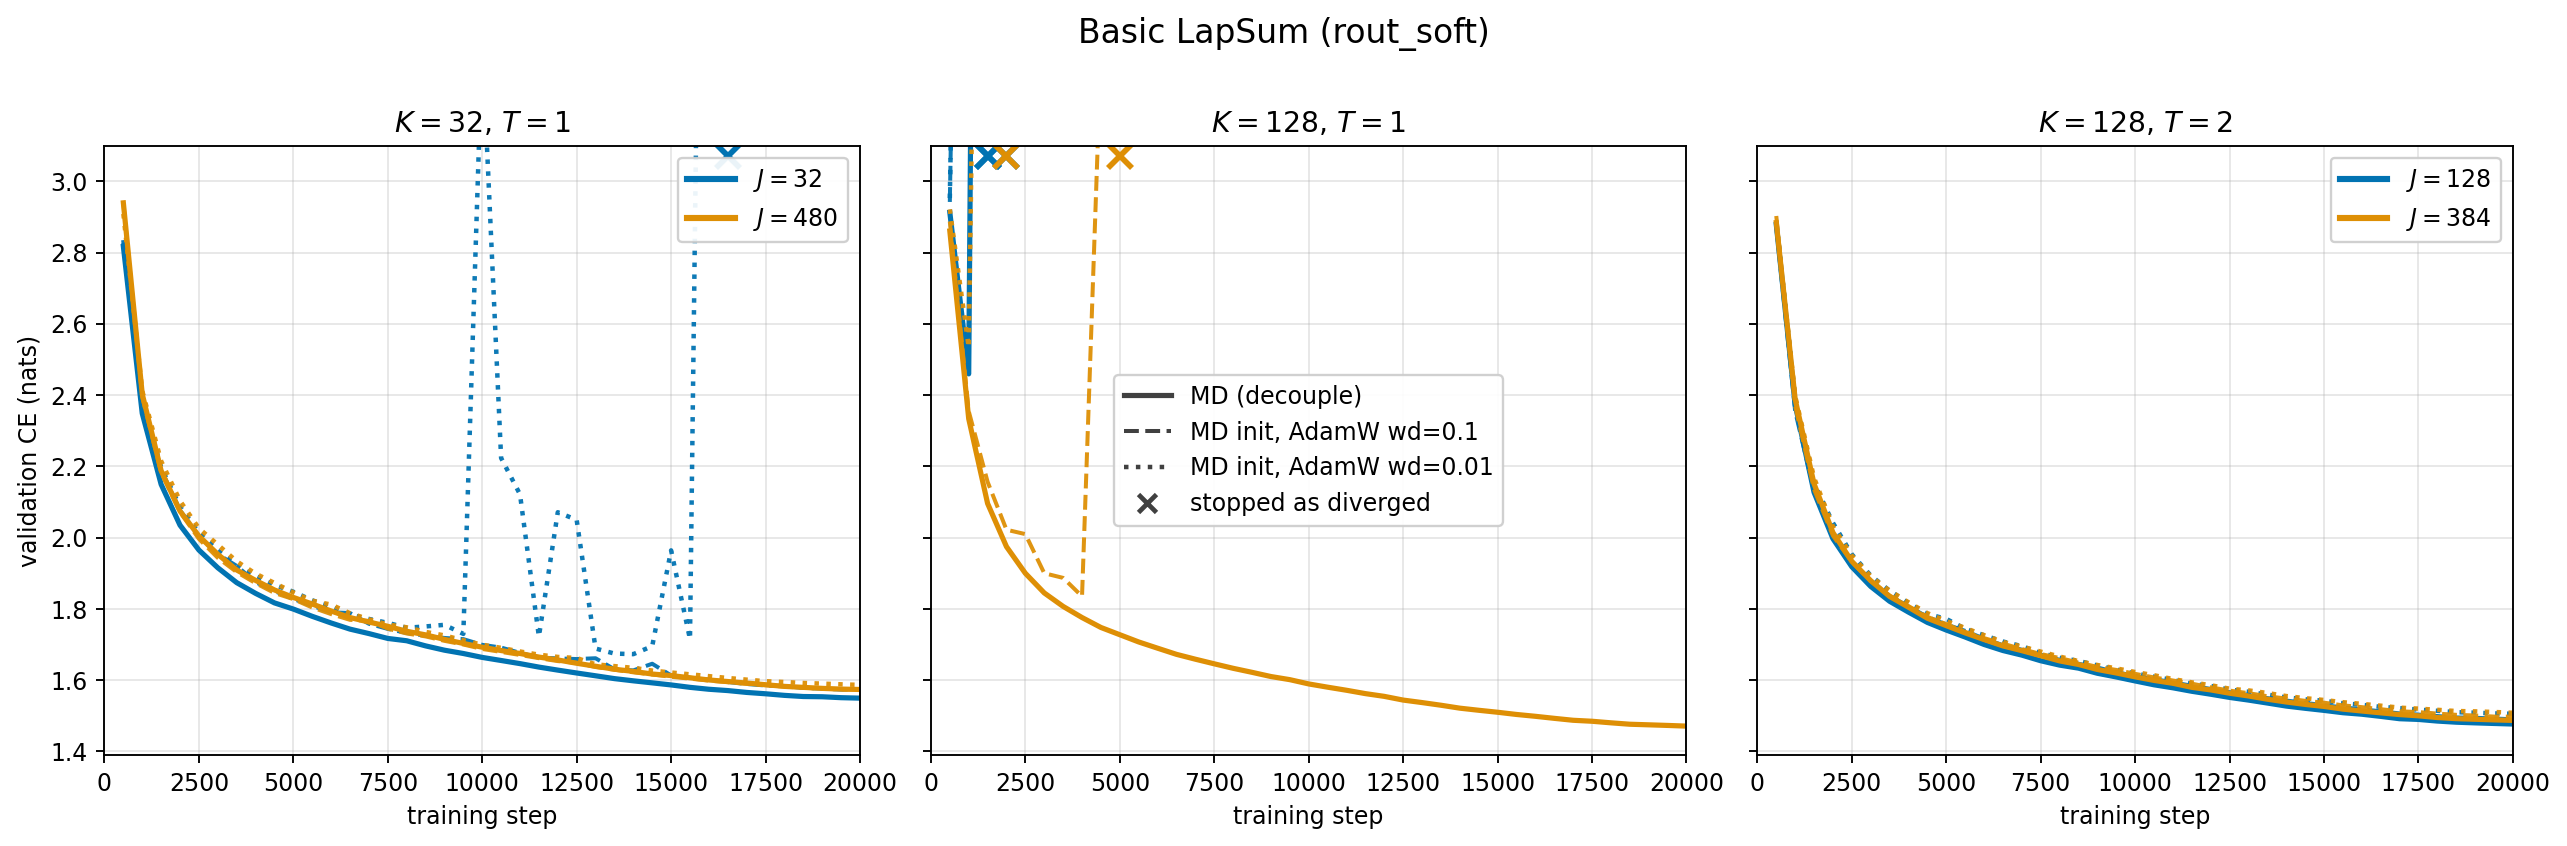
\includegraphics[width=\textwidth]{figures/mdinit_val_soft.png}
\caption{Validation CE for the basic LapSum family, split into panels
($K{=}32$, $T{=}1$), ($K{=}128$, $T{=}1$), ($K{=}128$, $T{=}2$). Within a
panel, color encodes $J$ and line style encodes the regime (full MD solid,
\code{md\_init} $wd{=}0.1$ dashed, $wd{=}0.01$ dotted). A cross marks the
point at which a run was stopped as diverged; crosses at the top edge belong
to curves that left the plotted range.}
\end{figure}

\begin{center}\small
\begin{tabular}{llccc}
\toprule
$(K,J)$ & $T$ & MD & \code{md\_init}, $wd{=}0.1$ & \code{md\_init}, $wd{=}0.01$ \\
\midrule
$(32,32)$   & 1 & 1.5497 & 1.5751 & \dv{16{,}700} \\
$(32,480)$  & 1 & 1.5740 & 1.5748 & 1.5868 \\
$(128,128)$ & 1 & \dv{2140} & \dv{1700} & \dv{1540} \\
$(128,128)$ & 2 & 1.4770 & 1.4904 & 1.5059 \\
$(128,384)$ & 1 & \textbf{1.4712} & \dv{5300} & \dv{2080} \\
$(128,384)$ & 2 & 1.4872 & 1.4978 & 1.5086 \\
\bottomrule
\end{tabular}
\end{center}

Final validation CE after 20k steps, or the step at which the divergence
guard stopped the run.

Two observations. First, in the four rows in which both regimes converge,
the \code{md\_init} curves track the MD curves closely throughout training;
the final gap to MD is $0.0008$--$0.025$ nats at $wd{=}0.1$ and
$0.013$--$0.029$ at $wd{=}0.01$. Second, the $(128,384)$, $T{=}1$ row
separates the regimes sharply: full MD converges to the best value in the
family, while both \code{md\_init} runs diverge.

% ============================================================
\section{Results: RBLapSum \texorpdfstring{\code{through\_rank\_kappa}}{through-rank-kappa}}
% ============================================================

\begin{figure}[h]\centering
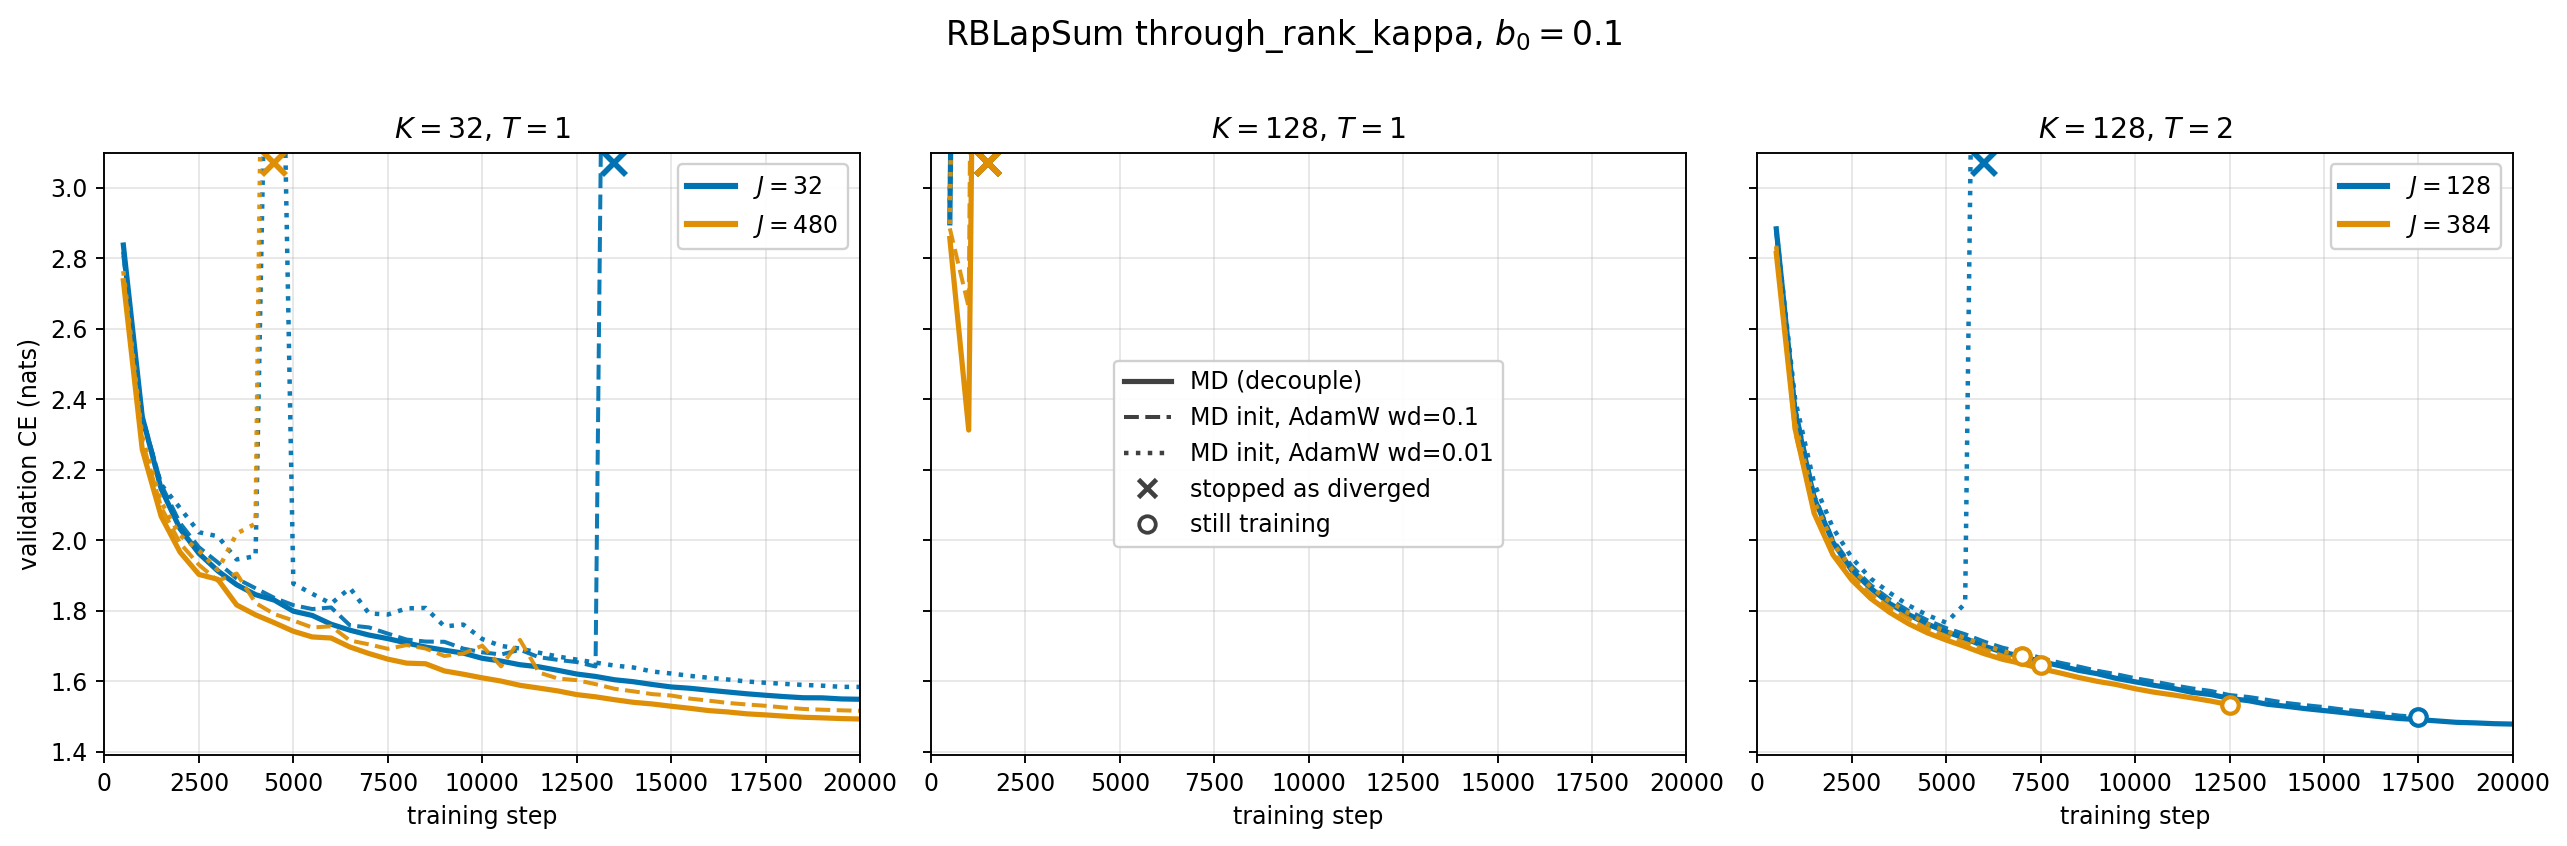
\includegraphics[width=\textwidth]{figures/mdinit_val_rblapsum_kappa.png}
\caption{Validation CE for the RBLapSum \code{through\_rank\_kappa} family,
panels as in the previous figure. An open circle marks the last available
point of a run still training at the time of this snapshot. In the middle
panel every run of both $(K,J)$ pairs diverges within the first
$\sim$2000 steps.}
\end{figure}

\begin{center}\small
\begin{tabular}{llccc}
\toprule
$(K,J)$ & $T$ & MD & \code{md\_init}, $wd{=}0.1$ & \code{md\_init}, $wd{=}0.01$ \\
\midrule
$(32,32)$   & 1 & 1.5482 & \dv{13{,}860} & 1.5833 \\
$(32,480)$  & 1 & 1.4923 & 1.5155 & \dv{5000} \\
$(128,128)$ & 1 & \dv{1760} & \dv{1720} & \dv{1540} \\
$(128,128)$ & 2 & 1.4778 & 1.538 at 14k (running) & \dv{6460} \\
$(128,384)$ & 1 & \dv{1880} & \dv{1800} & \dv{1640} \\
$(128,384)$ & 2 & 1.590 at 9.5k (running) & 1.748 at 4.5k (running) & 1.826 at 3.5k (running) \\
\bottomrule
\end{tabular}
\end{center}

The same pattern with more divergences, consistent with this family's known
narrower stability region at $T=1$. Full MD again diverges only in the two
rows in which everything diverges. \code{md\_init} additionally loses
$(32,32)$ at $wd{=}0.1$ (a late death at step 13{,}860 after repeated
recovering bursts), $(32,480)$ at $wd{=}0.01$, and $(128,128)$, $T{=}2$ at
$wd{=}0.01$; in the surviving comparable pairs the final gap to MD is
$0.023$--$0.035$ nats.

% ============================================================
\section{Results: hard AbsTopK}
% ============================================================

\begin{figure}[h]\centering
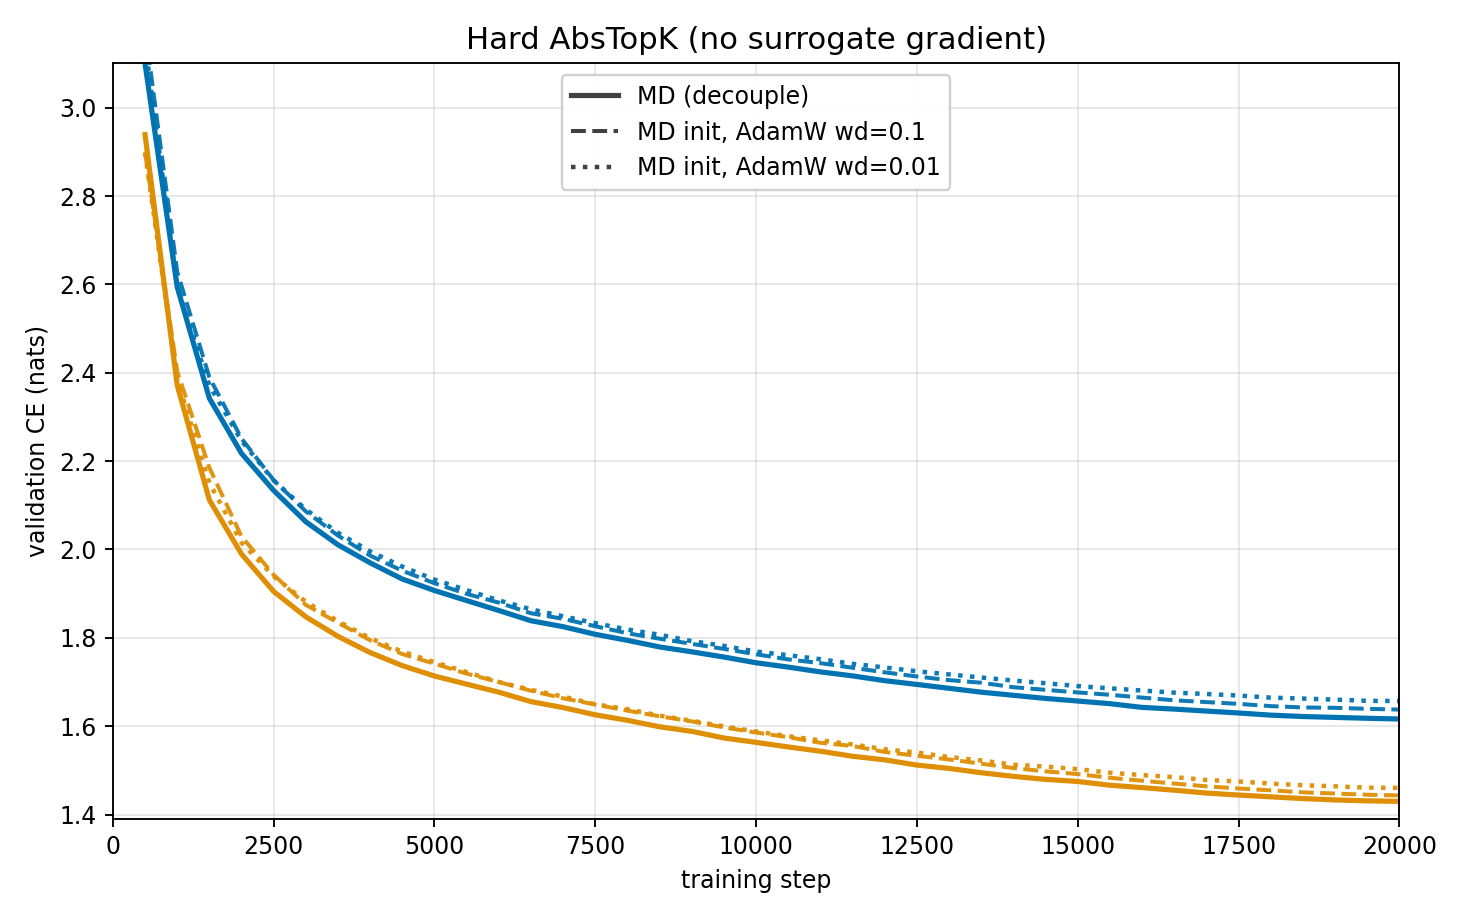
\includegraphics[width=.94\textwidth]{figures/mdinit_val_hard.png}
\caption{Validation CE for the hard AbsTopK family (no surrogate
gradient); color encodes $K$. No run in this family diverged.}
\end{figure}

\begin{center}\small
\begin{tabular}{lccc}
\toprule
$K$ & MD & \code{md\_init}, $wd{=}0.1$ & \code{md\_init}, $wd{=}0.01$ \\
\midrule
$32$  & 1.6162 & 1.6375 & 1.6569 \\
$512$ & 1.4298 & 1.4432 & 1.4605 \\
\bottomrule
\end{tabular}
\end{center}

With no surrogate gradient there are no divergences, and the comparison is
purely about quality. The ordering MD $<$ $wd{=}0.1$ $<$ $wd{=}0.01$ holds at
both $K$, with gaps to MD of $0.013$--$0.021$ nats at $wd{=}0.1$ and
$0.031$--$0.041$ at $wd{=}0.01$.

% ============================================================
\section{Conclusions}
% ============================================================

\begin{enumerate}[leftmargin=1.6em]
\item \textbf{The initialization carries most of the converged quality.}
Ordinary AdamW started from the MD initialization reaches within
$0.001$--$0.025$ nats of full MD at $wd{=}0.1$ in every configuration in
which both converge, across all three families. If MD training is adopted
for its final loss on stable configurations, most of that benefit is
available from the initialization (with its $\sqrt d$ embedding upscale)
alone.

\item \textbf{The decoupling itself is what buys stability.} Every
configuration lost by full MD was lost by all three regimes, whereas
\code{md\_init} diverged in six additional cells spread over both surrogate
families, both $(K,J)$ extremes, and both weight decays. In rows in which
all three regimes diverge, the death order is systematically $wd{=}0.01$
first, $wd{=}0.1$ second, MD last. The norm constraint does not eliminate
the $K=128$, $T=1$ instability, but it consistently delays it and widens the
set of configurations that survive 20k steps.

\item \textbf{Full MD retains a small, consistent quality edge} of
$0.001$--$0.041$ nats over \code{md\_init} in every completed pair. The edge
grows with the weaker weight decay, so part of it is attributable to the
regularization difference rather than to the geometry of the update.

\item \textbf{Scope.} All cells are single runs at one seed. Earlier work in
this project showed that divergence at marginal configurations is
stochastic, so individual cell outcomes should be read as draws from a
divergence rate; the row-level patterns (all-regime deaths at $K{=}128$,
$T{=}1$; the systematic death ordering; MD never diverging alone) are the
robust part. Four runs (marked ``running'') had not finished at the time of
writing; the tables and figures will be updated when they complete.
\end{enumerate}

\end{document}
